
\subsection*{task 2.6 \\[1ex] ``simple'' tiling effects}

Speaking of tiles of size $m \times n$, can you think of a piece of code that creates images like these where tiles have been moved around randomly? 
\begin{figure}[h!]
\subfloat[input image]{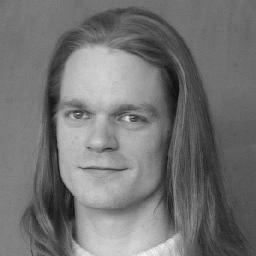
\includegraphics[width=0.24\textwidth]{portrait.png}} \hfill
\subfloat[tile size $8 \times 8$]{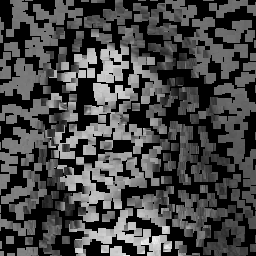
\includegraphics[width=0.24\textwidth]{t2-6-8x8.png}} \hfill
\subfloat[tile size $32 \times 32$]{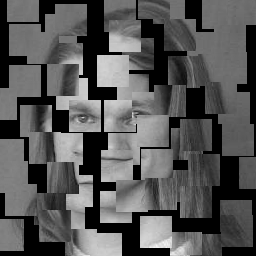
\includegraphics[width=0.24\textwidth]{t2-6-32x32.png}} \hfill
\subfloat[tile size $13 \times 7$]{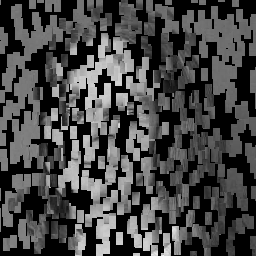
\includegraphics[width=0.24\textwidth]{t2-6-13x7.png}} \hfill
\end{figure}

\textbf{Note:} the example with the $13 \times 7$ tiles is just to show off \ldots for your own solution, you may simply focus on square input images and square tiles whose side lengths are proper divisors of the side lengths of the image.

\textbf{Note:} \emph{numpy} code for the above effect can again be realized without any \keyword{for} loops \ldots However, this requires truly advanced insights into the capabilities of \emph{numpy} and has nothing to do with understanding how image processing works. You can therefore devise an intuitive solution with as many \keyword{for} loops as you deem necessary. (But brace yourself for likely slow execution times.)

Paste your code here %\\[1ex]
%%%%%
%%%%%
%%%%% enter your code into the following environment
%%%%%
%%%%%
\begin{python}
# paste your code here

\end{python}
%%%%%
%%%%%
%%%%%
%%%%%
%%%%%
